% Diagramas e contratos do item 4(c). Incluido por main.tex.
\clearpage
\subsection{Diagramas de Sequência do Sistema}
\label{ap:dss}

As Figuras~\ref{fig:dss-uc03}--\ref{fig:dss-uc09} apresentam as
mensagens observáveis dos seis casos de uso centrais. O serviço de
pagamento é mostrado como ator externo no UC08, sem detalhar a
implementação dos componentes internos do DevMatch.

\begin{figure*}[!p]
\centering
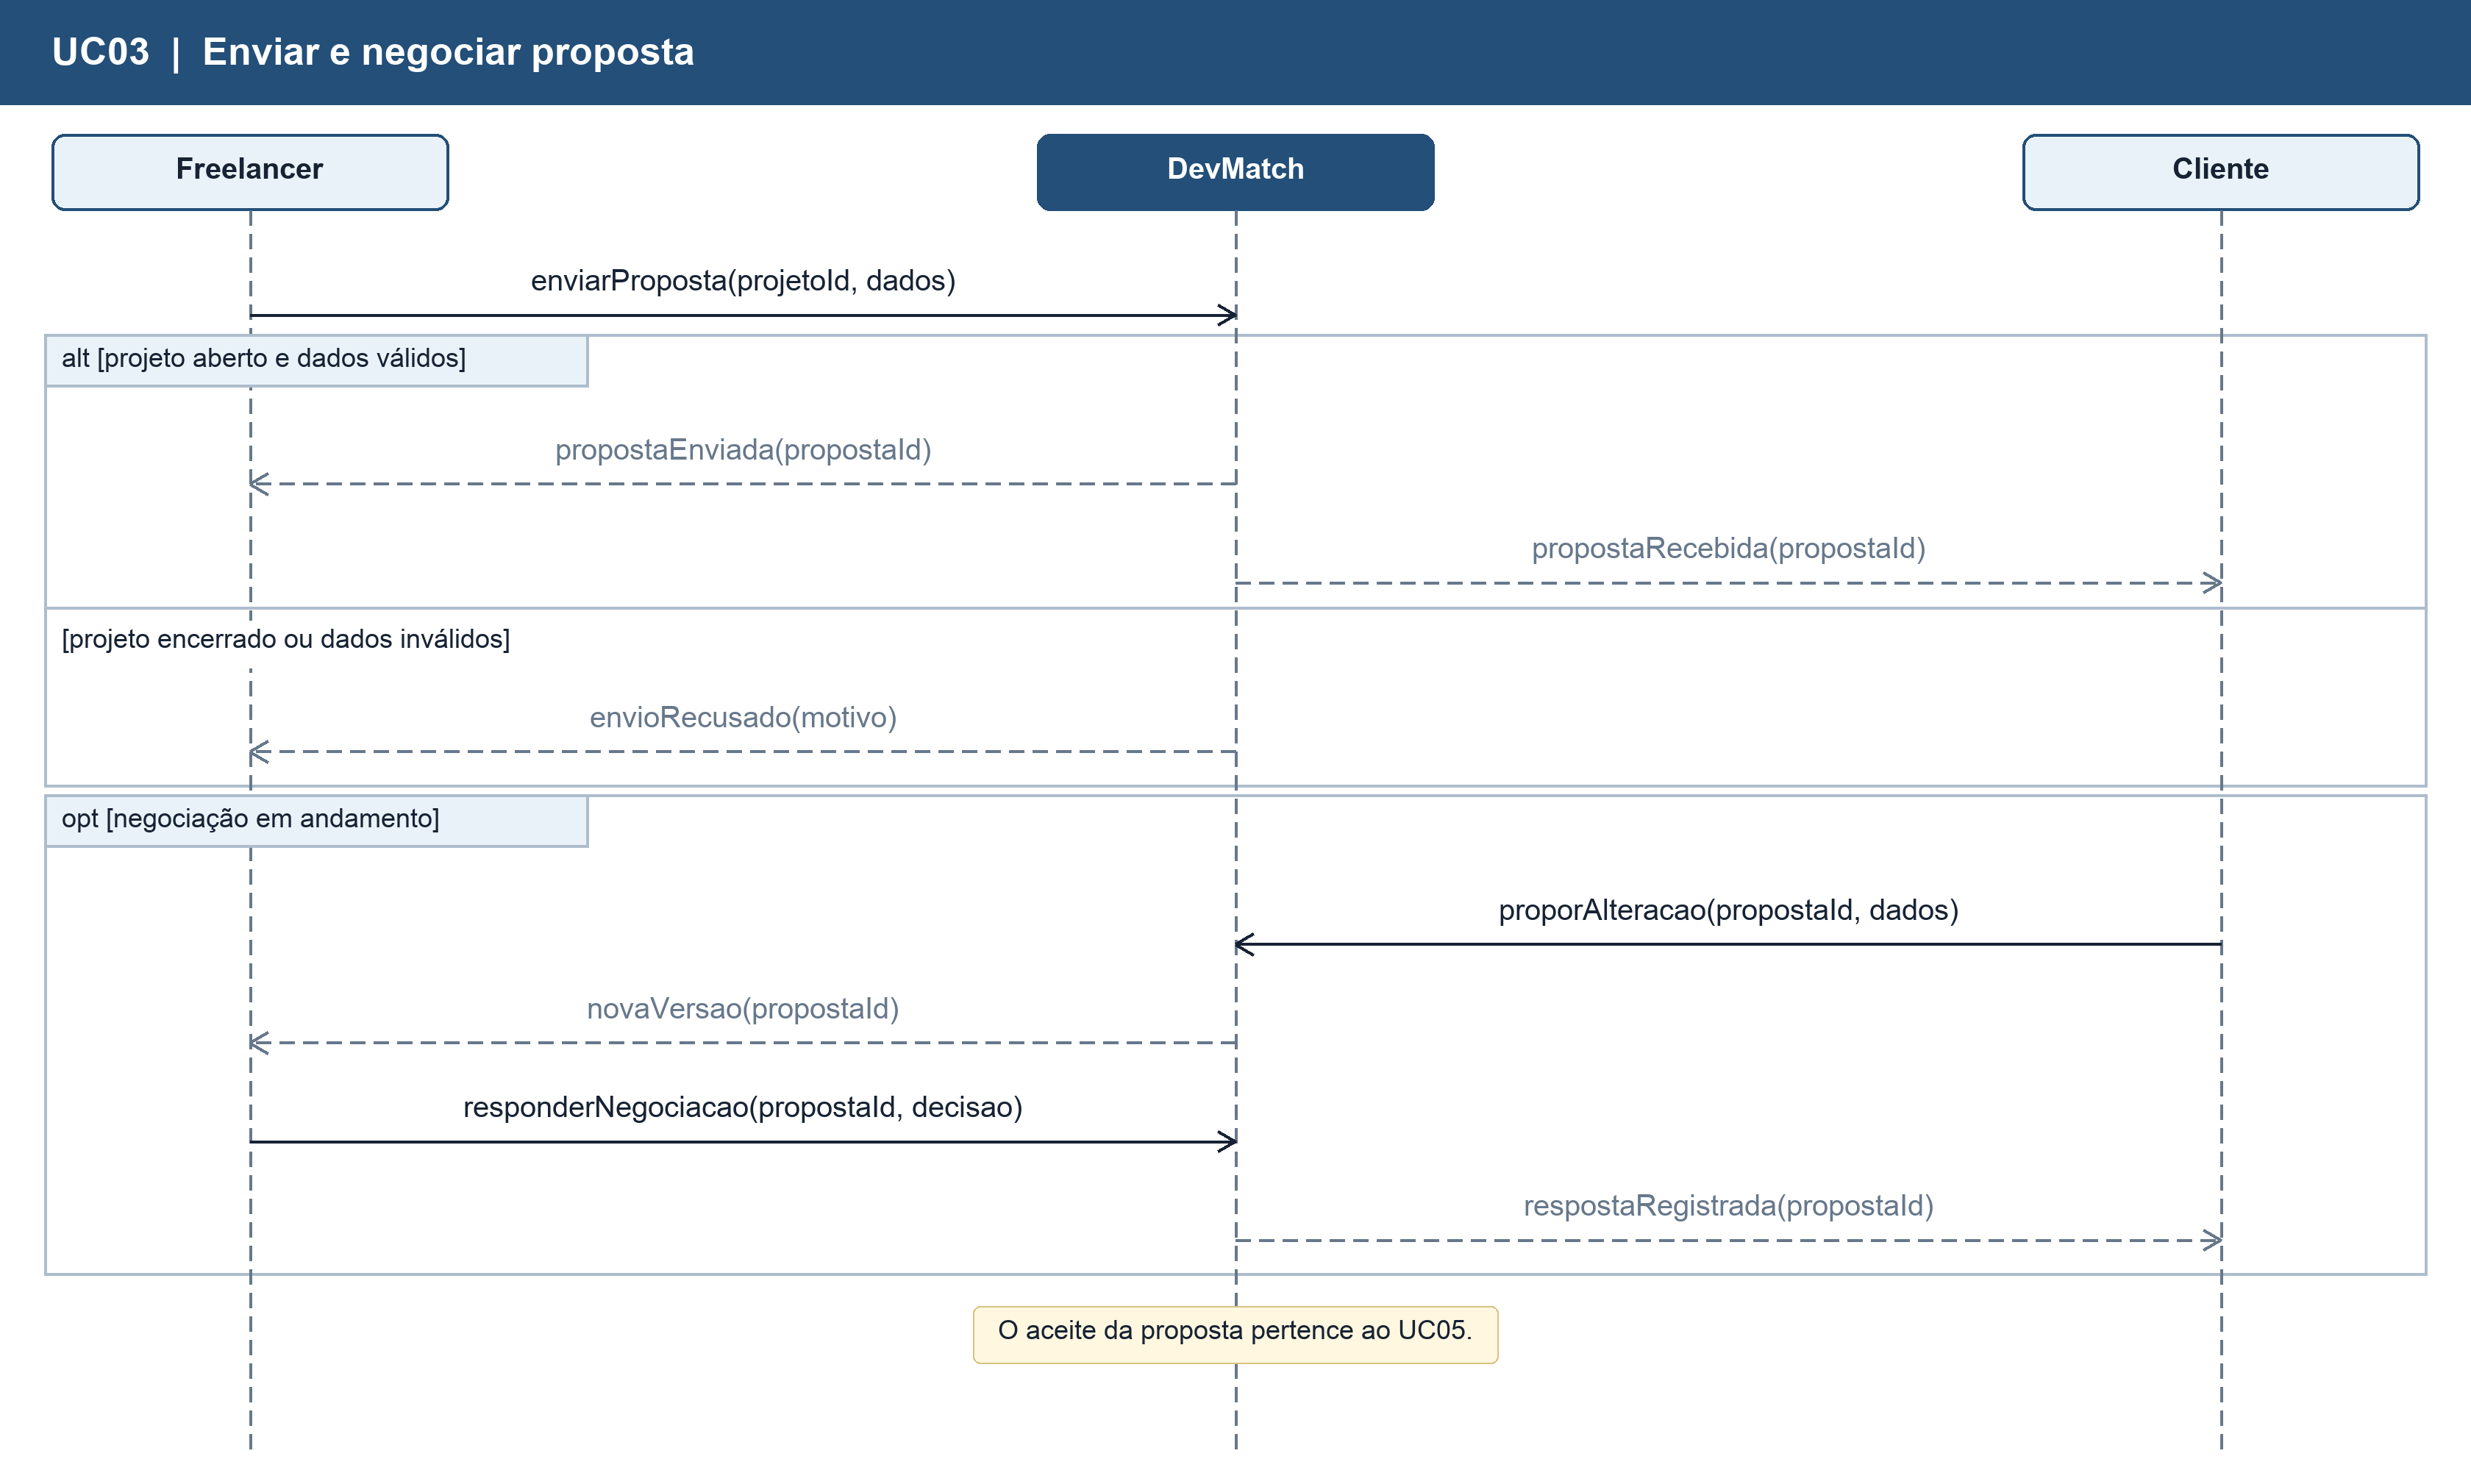
\includegraphics[width=\textwidth,height=0.80\textheight,keepaspectratio]{diagramas/dss_uc03.png}
\caption{DSS do UC03: envio e negociação de proposta.}
\label{fig:dss-uc03}
\end{figure*}

\begin{figure*}[!p]
\centering
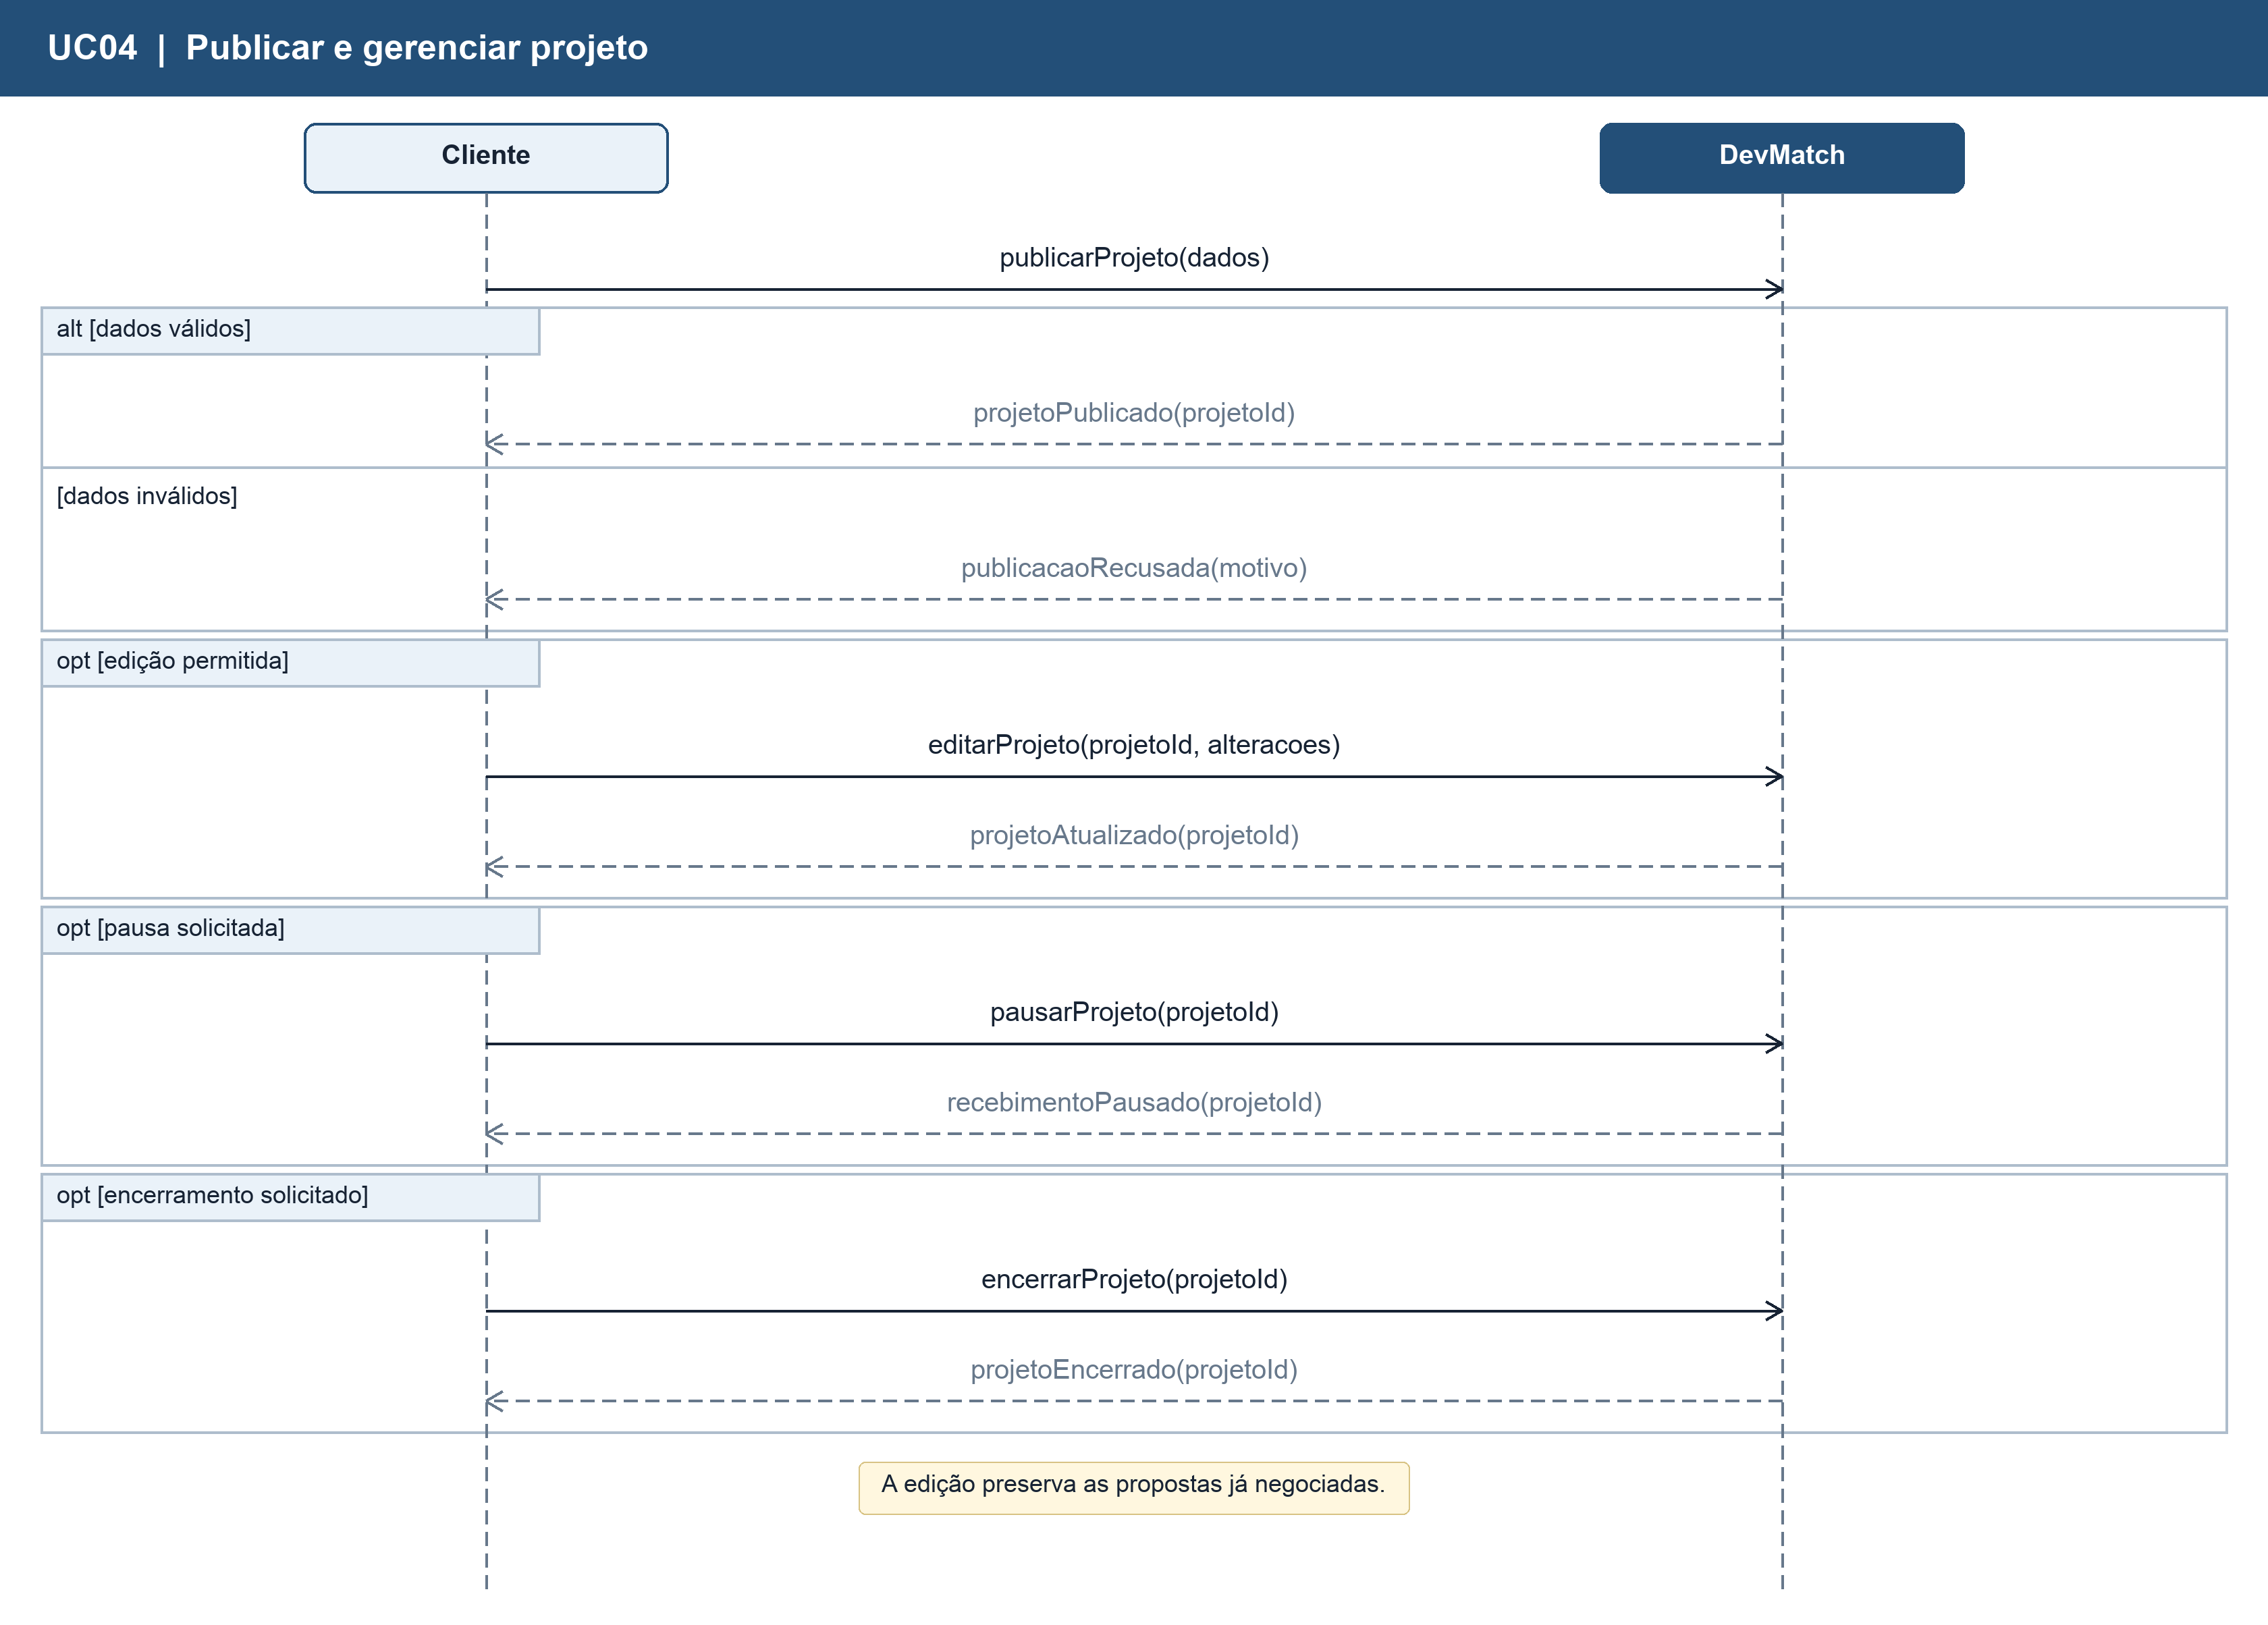
\includegraphics[width=\textwidth,height=0.80\textheight,keepaspectratio]{diagramas/dss_uc04.png}
\caption{DSS do UC04: publicação e gerenciamento de projeto.}
\label{fig:dss-uc04}
\end{figure*}

\begin{figure*}[!p]
\centering
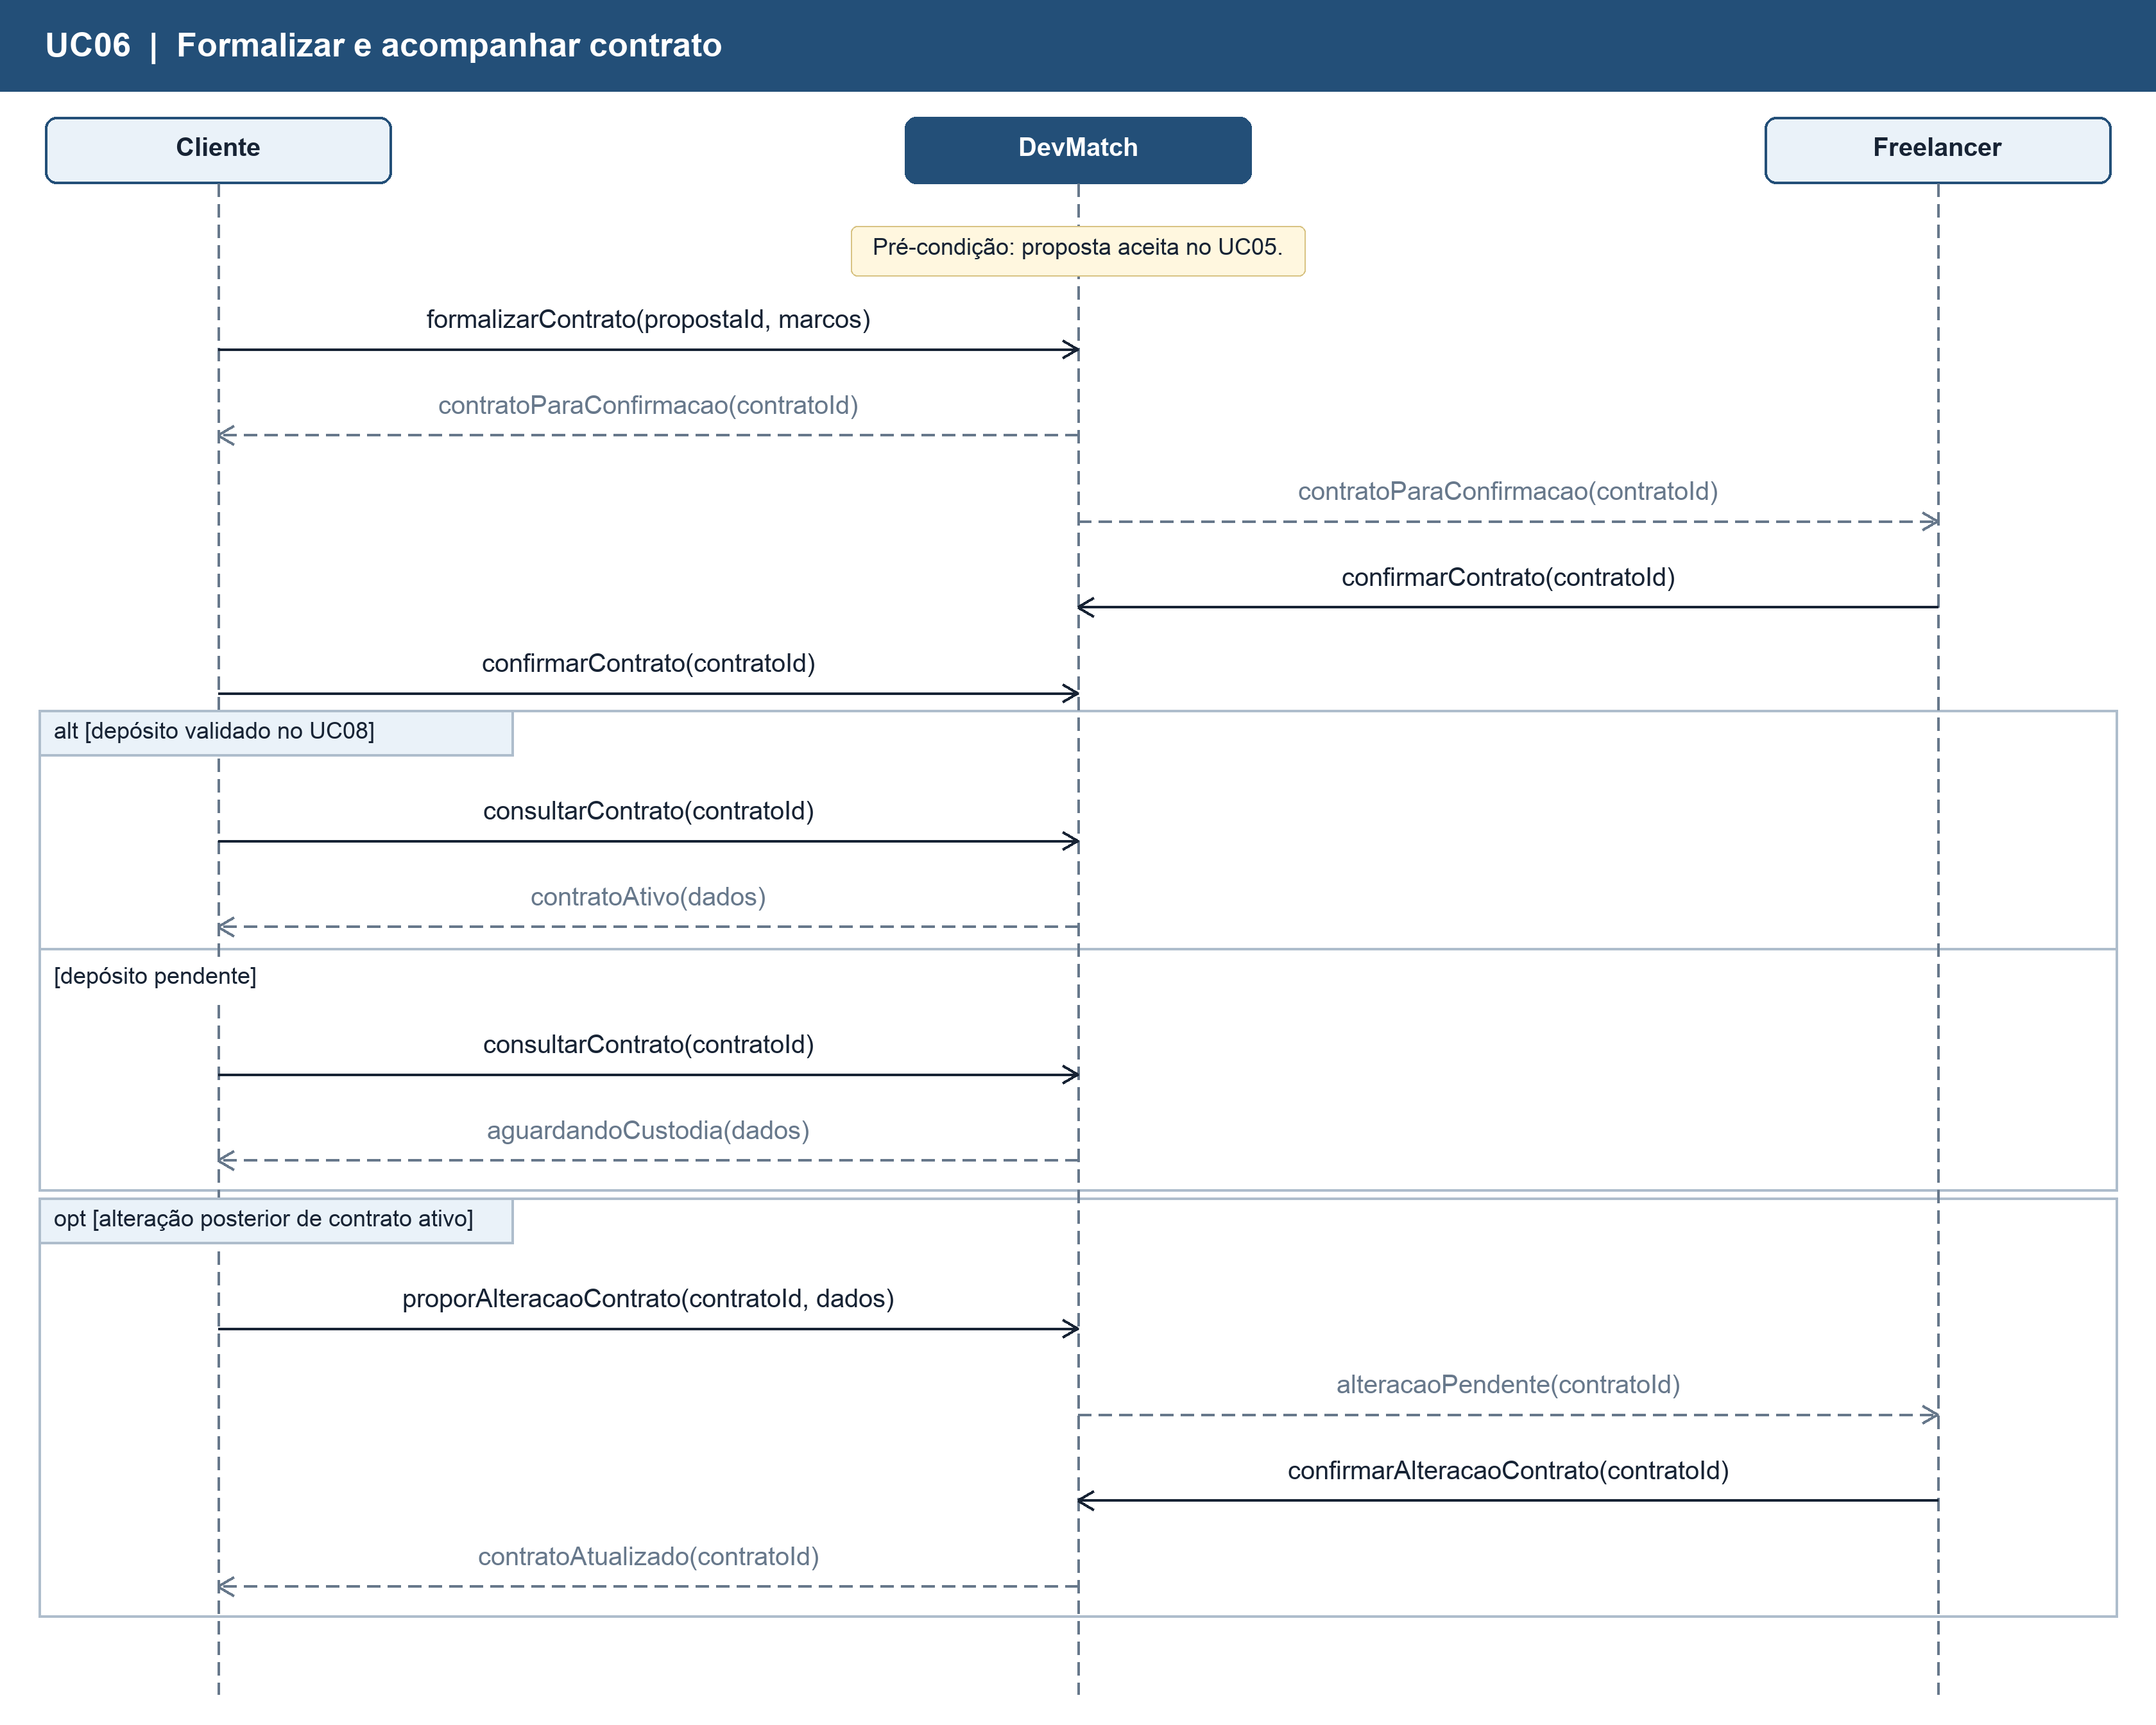
\includegraphics[width=\textwidth,height=0.80\textheight,keepaspectratio]{diagramas/dss_uc06.png}
\caption{DSS do UC06: formalização e acompanhamento de contrato.}
\label{fig:dss-uc06}
\end{figure*}

\begin{figure*}[!p]
\centering
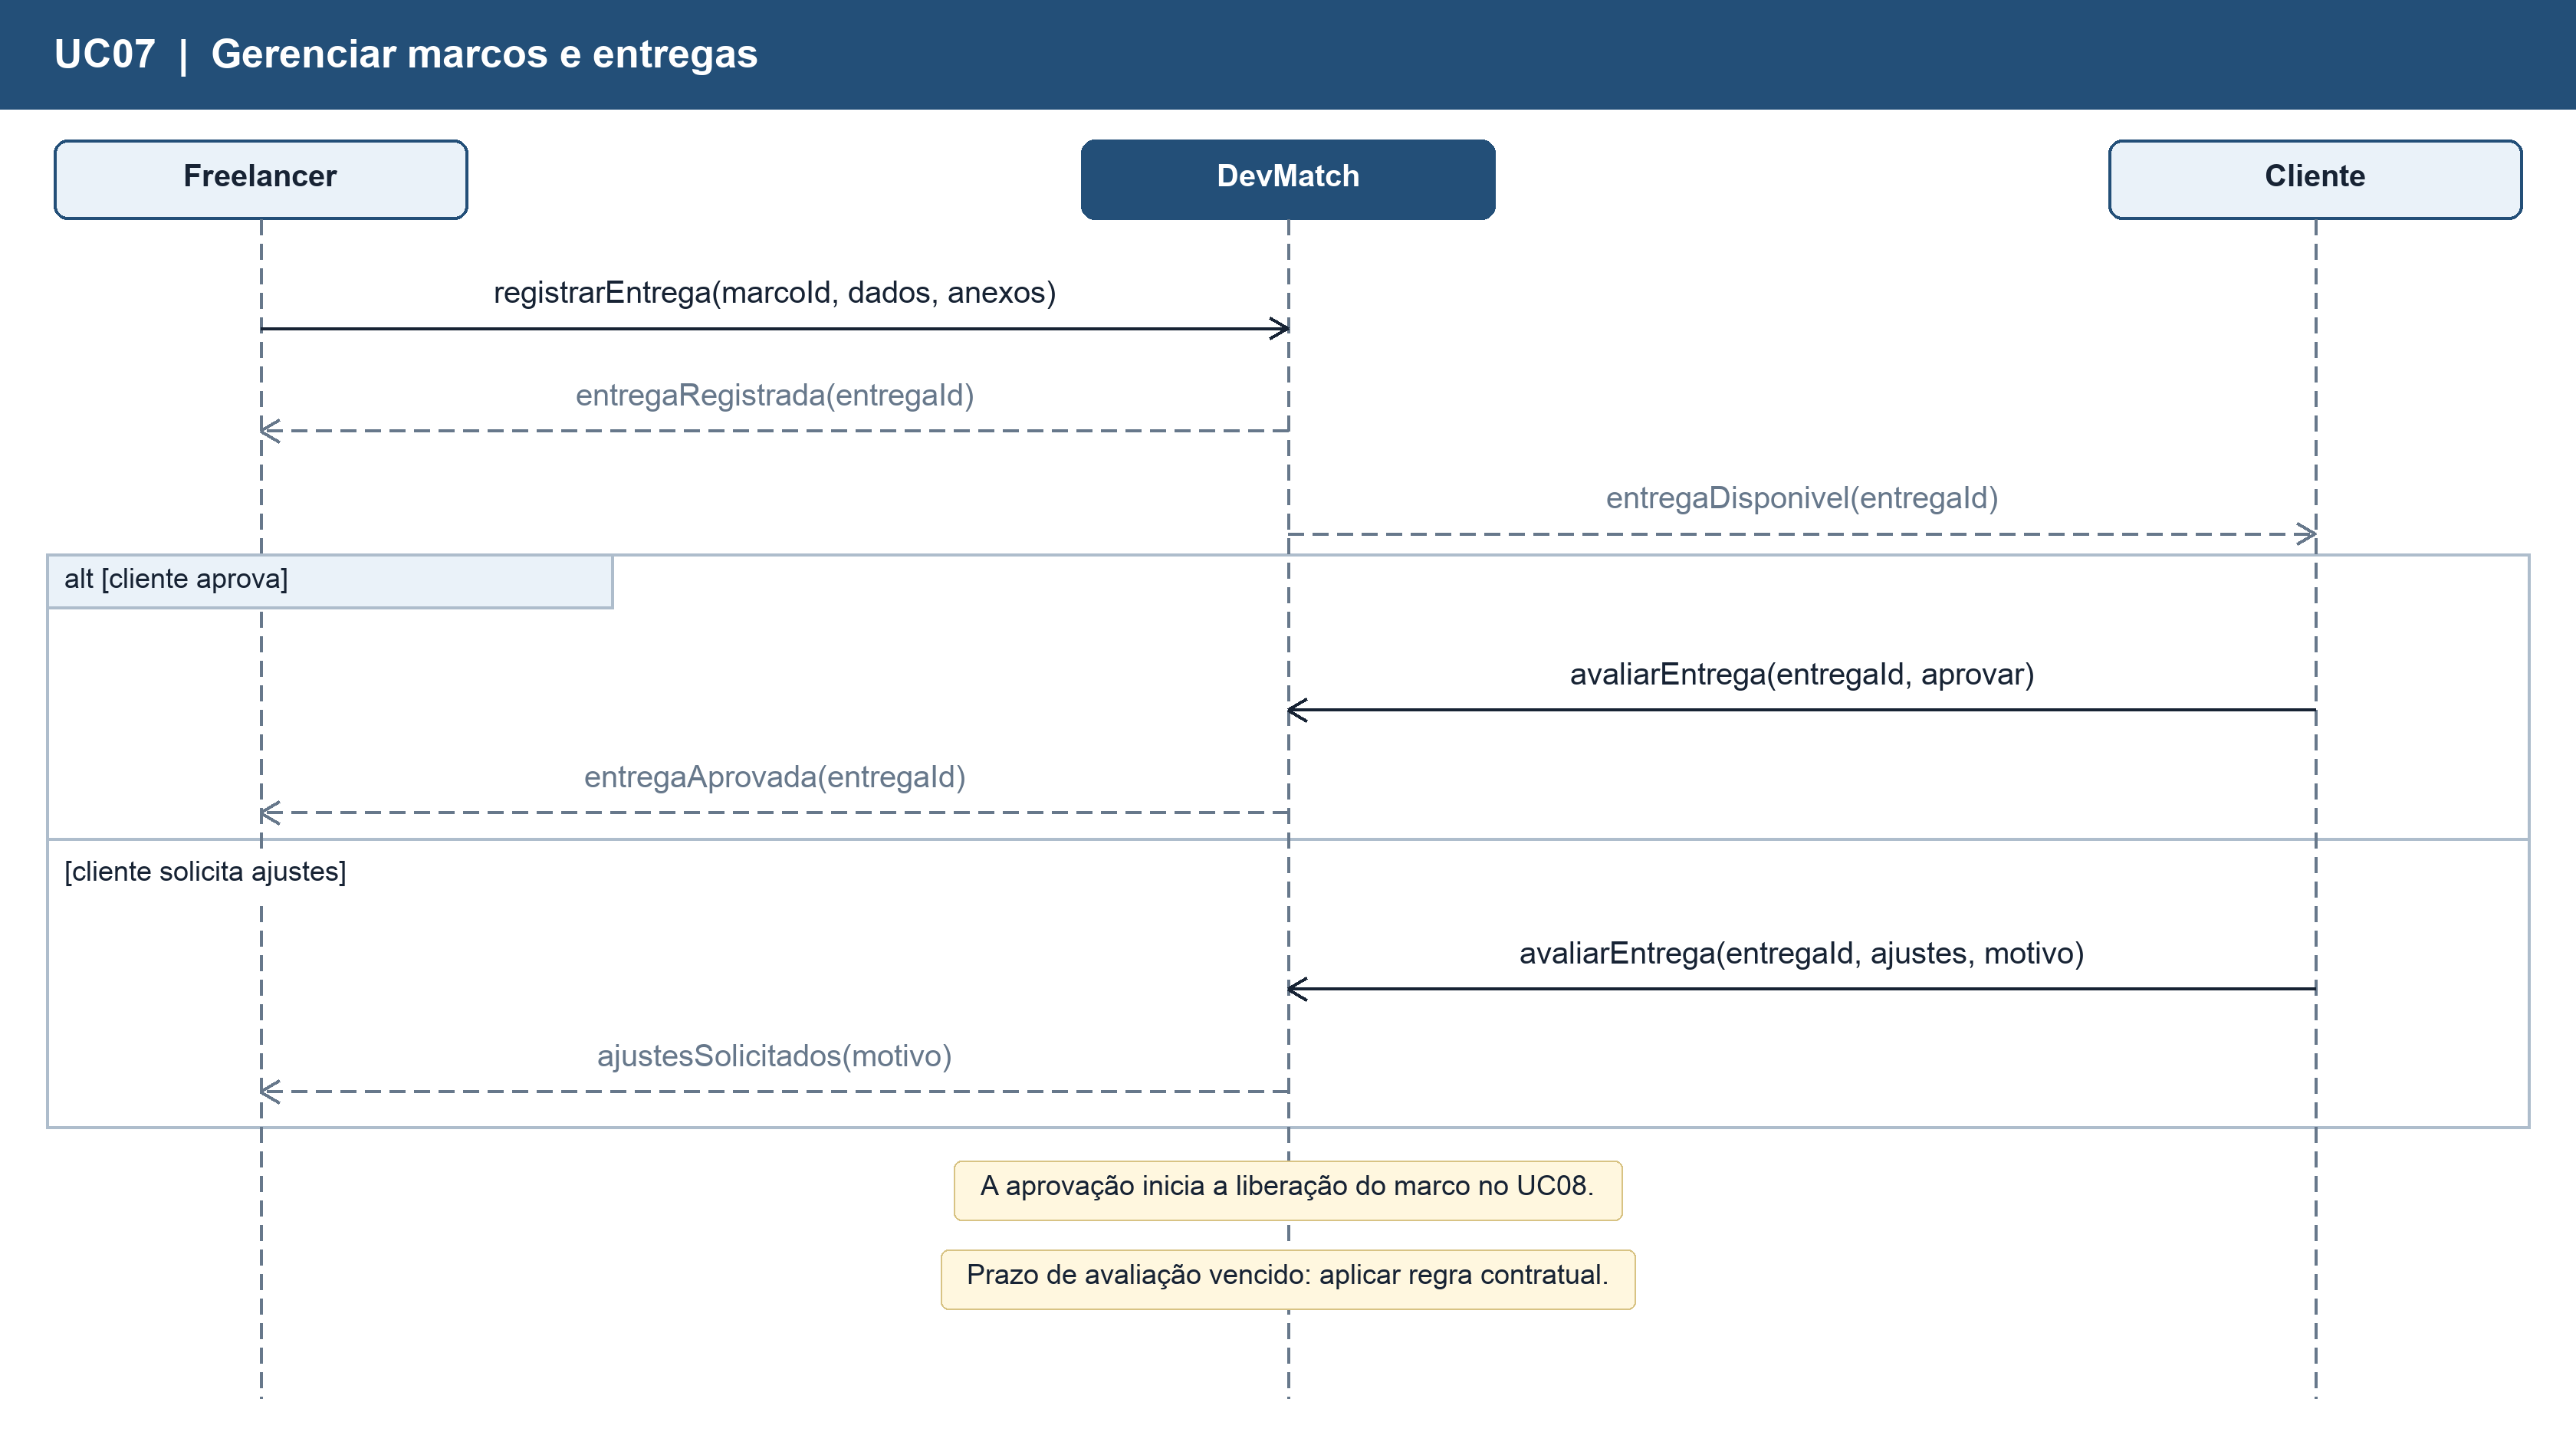
\includegraphics[width=\textwidth,height=0.80\textheight,keepaspectratio]{diagramas/dss_uc07.png}
\caption{DSS do UC07: gerenciamento de marcos e entregas.}
\label{fig:dss-uc07}
\end{figure*}

\begin{figure*}[!p]
\centering
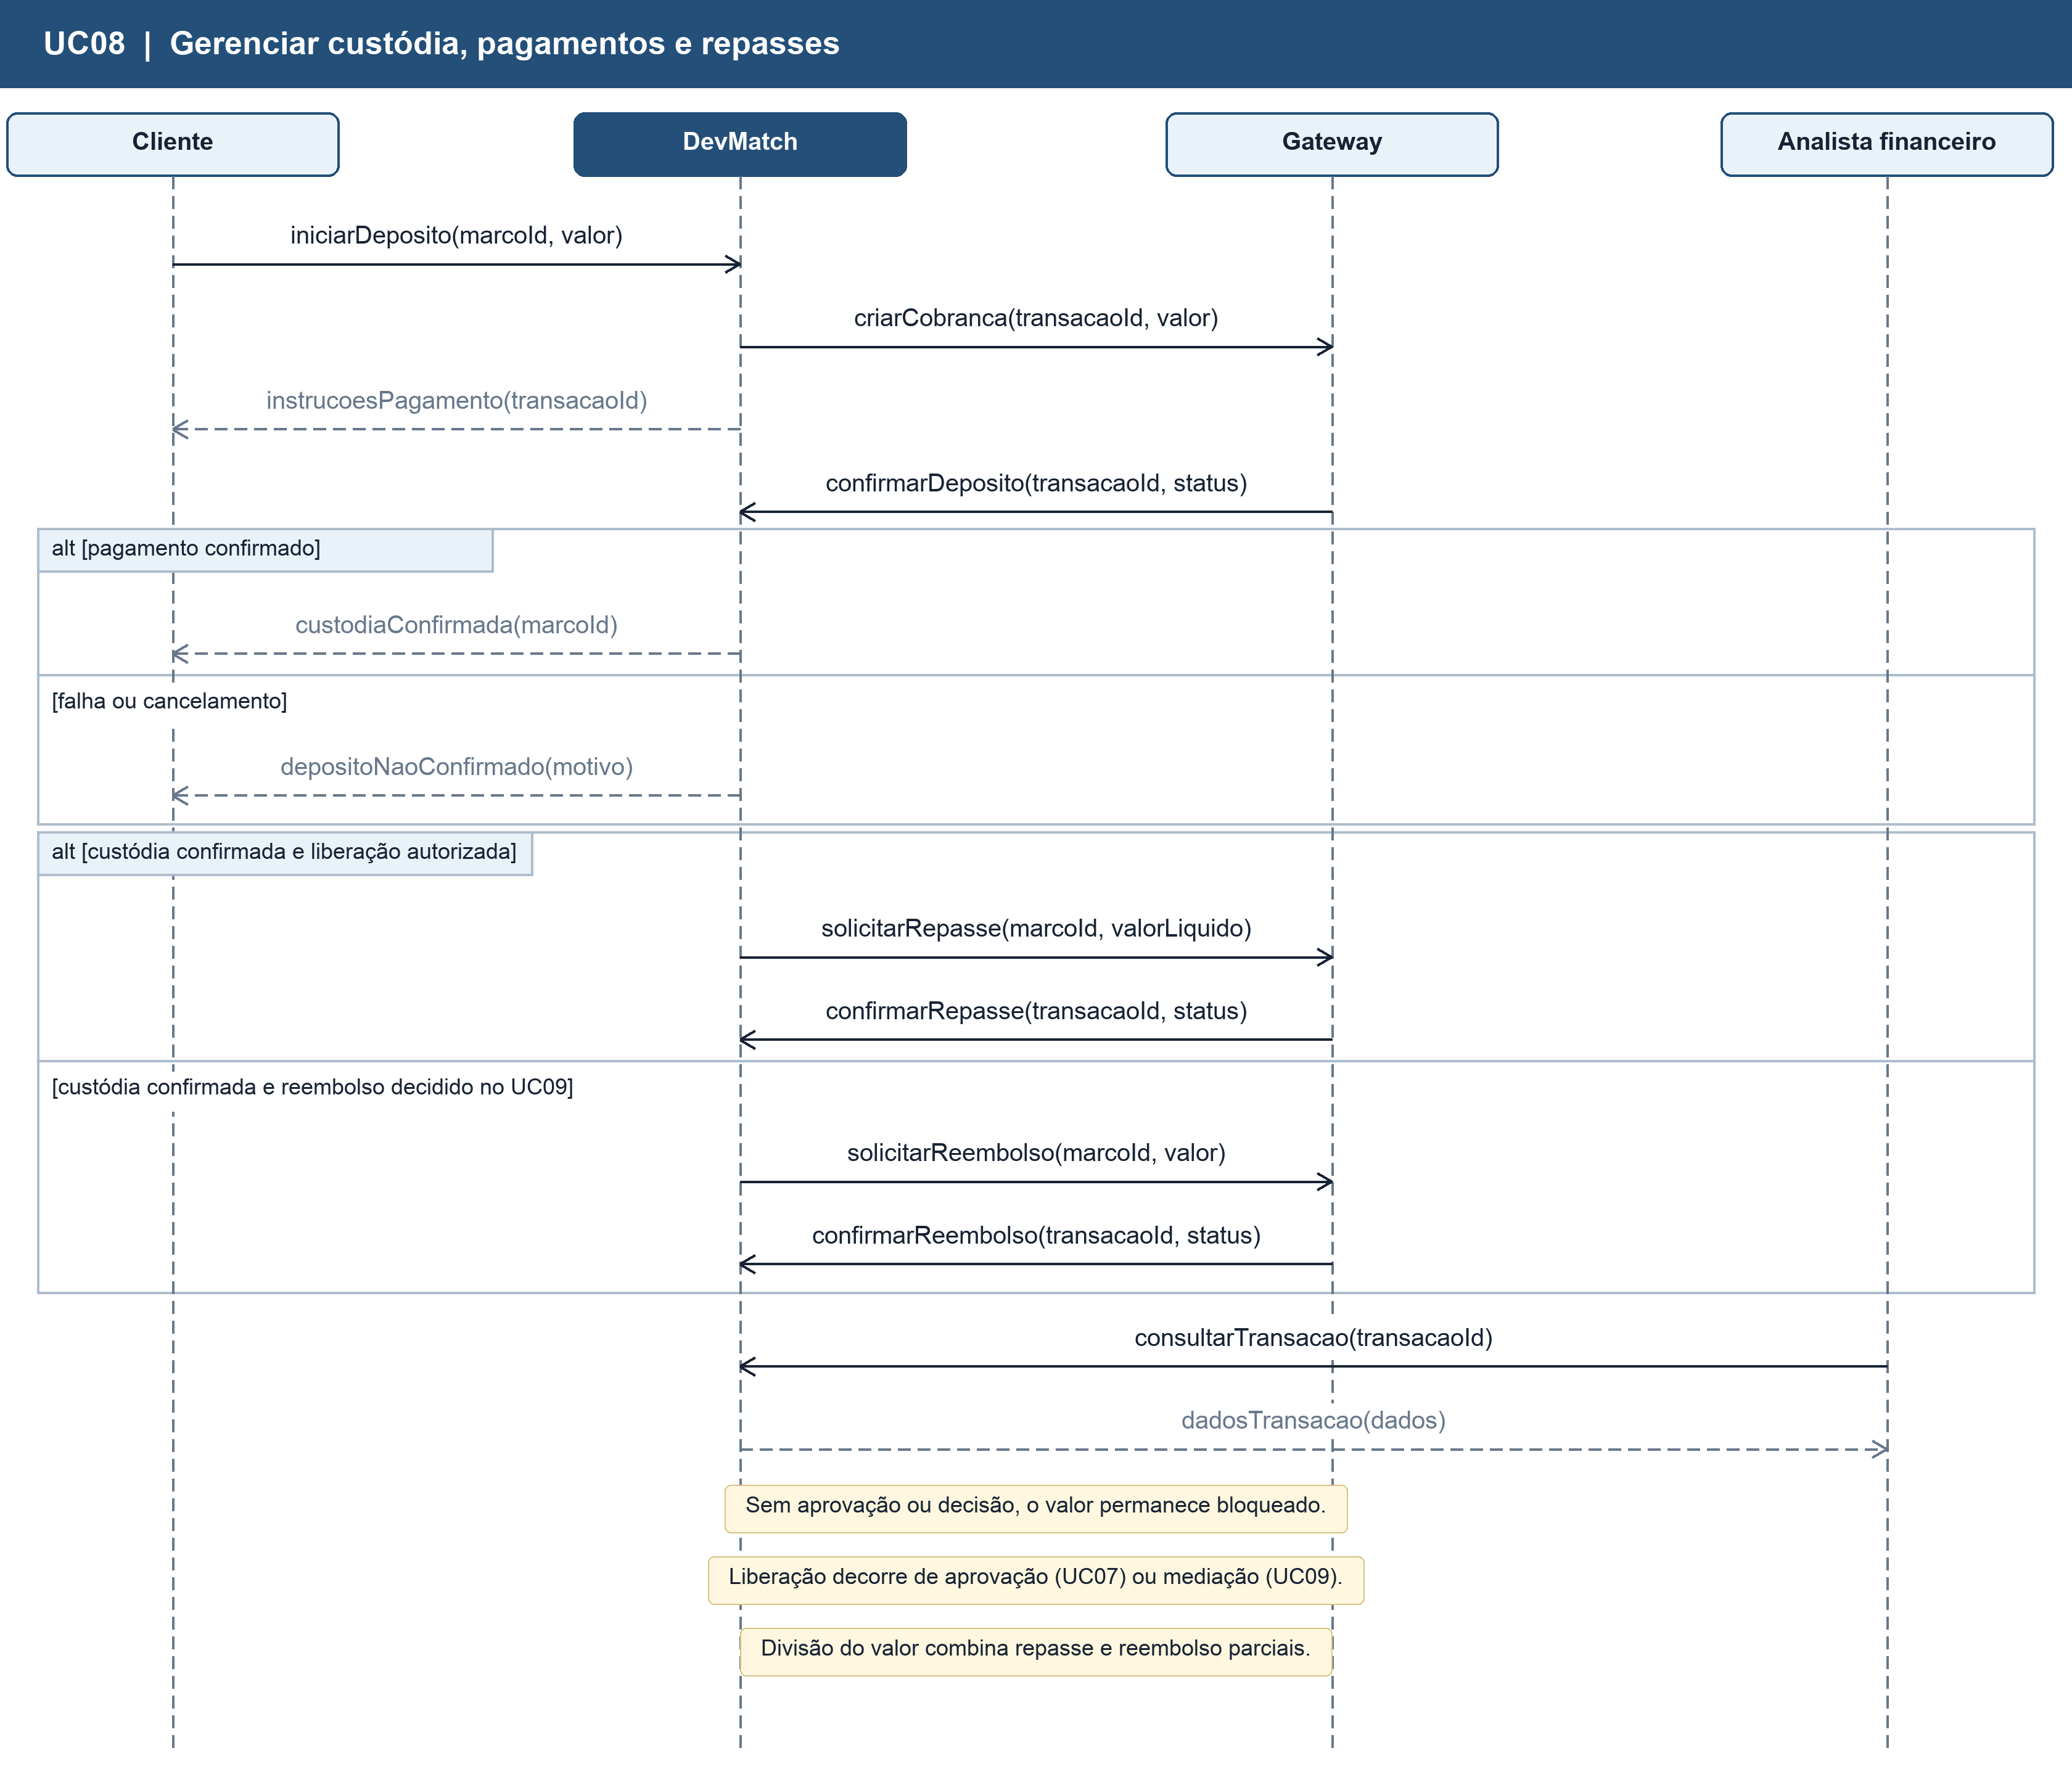
\includegraphics[width=\textwidth,height=0.80\textheight,keepaspectratio]{diagramas/dss_uc08.png}
\caption{DSS do UC08: custódia, pagamentos e repasses.}
\label{fig:dss-uc08}
\end{figure*}

\begin{figure*}[!p]
\centering
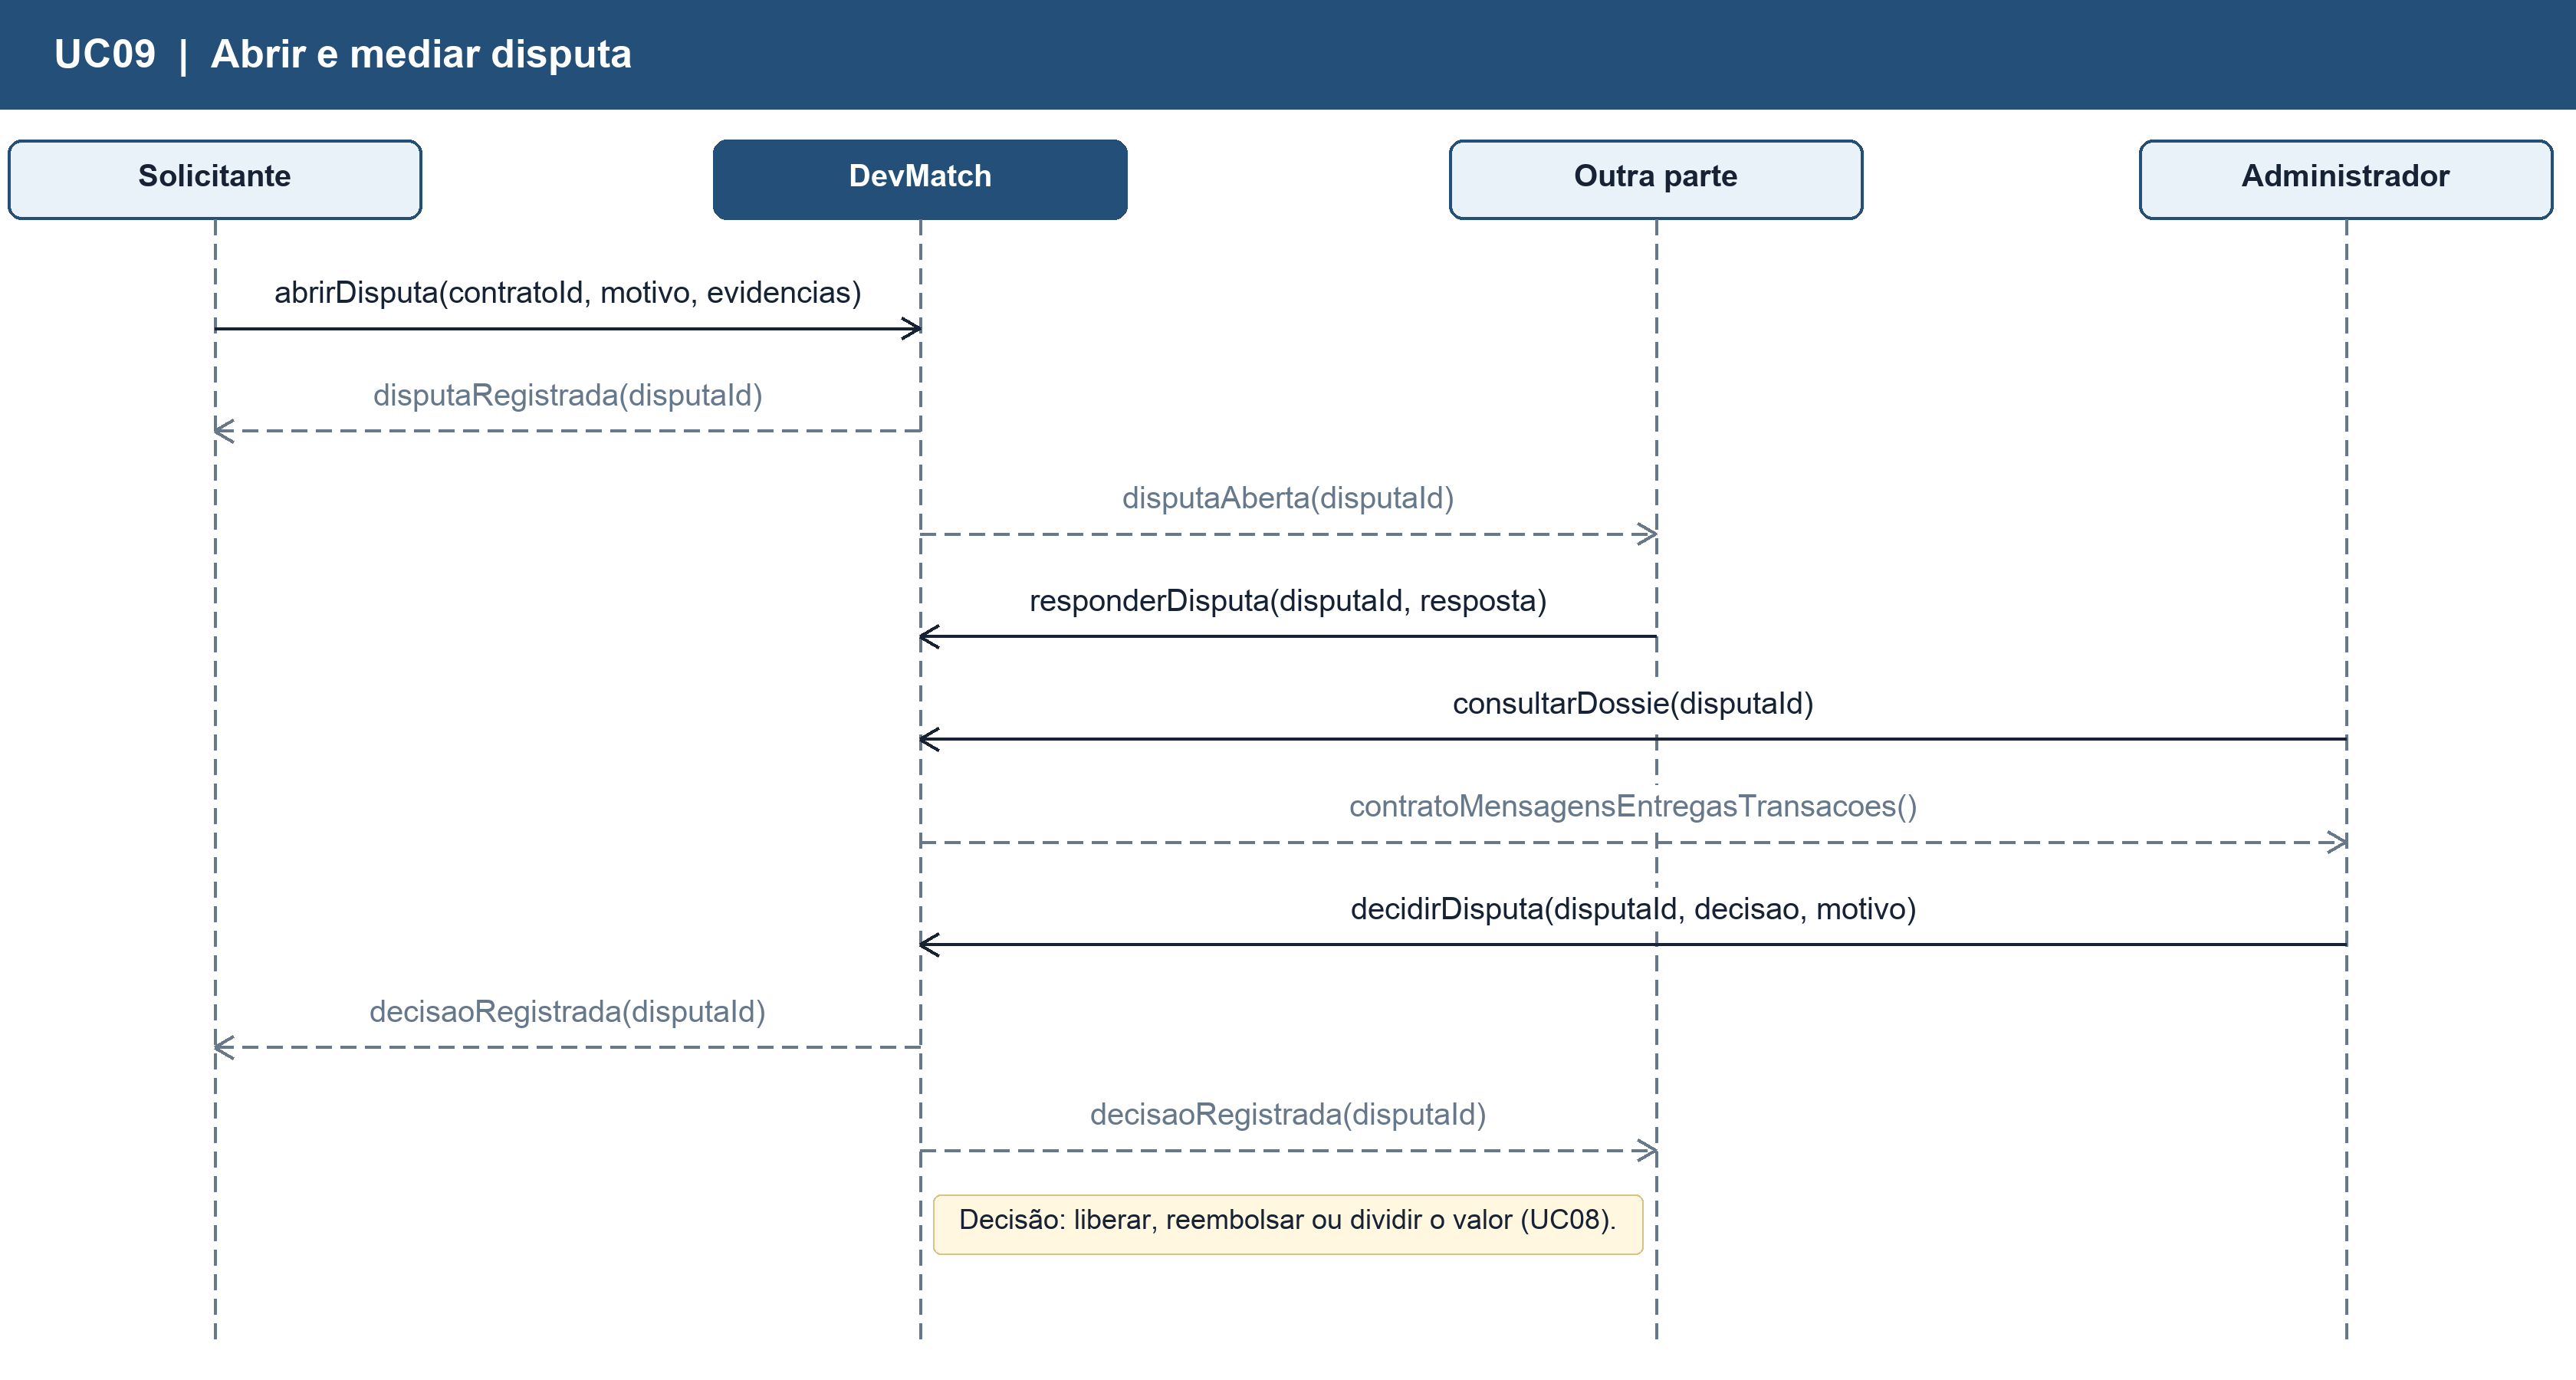
\includegraphics[width=\textwidth,height=0.80\textheight,keepaspectratio]{diagramas/dss_uc09.png}
\caption{DSS do UC09: abertura e mediação de disputa.}
\label{fig:dss-uc09}
\end{figure*}

\clearpage
\subsection{Contratos de Operação dos Casos Centrais}
\label{ap:contratos-operacao}

Os contratos a seguir descrevem o estado necessário antes de cada
operação e os efeitos observáveis depois de sua execução bem-sucedida.
Quando uma pré-condição ou validação não é atendida, o sistema devolve
o motivo da recusa e não produz o efeito de negócio indicado.

\subsubsection{UC03 -- Enviar e negociar proposta}

\paragraph{\texttt{enviarProposta}.}
\textit{Pré-condições:} freelancer autenticado, perfil ativo e projeto
aberto para propostas. \textit{Pós-condições:} uma proposta com valor,
prazo e observações válidos é registrada com identificador e estado
``enviada''; o cliente é notificado.

\paragraph{\texttt{proporAlteracao}.}
\textit{Pré-condições:} solicitante participa da negociação e a
proposta não está encerrada. \textit{Pós-condições:} uma nova versão
dos termos é registrada, o histórico anterior é preservado e a outra
parte é notificada.

\paragraph{\texttt{responderNegociacao}.}
\textit{Pré-condições:} destinatário autorizado e versão pendente de
resposta. \textit{Pós-condições:} a resposta e a situação da
negociação são registradas, com preservação das versões. A seleção
do freelancer para contratação permanece no UC05.

\subsubsection{UC04 -- Publicar e gerenciar projeto}

\paragraph{\texttt{publicarProjeto}.}
\textit{Pré-condições:} cliente autenticado; título, escopo,
orçamento, prazo, tecnologias e critérios de aceitação informados.
\textit{Pós-condições:} o projeto validado recebe identificador,
fica aberto para propostas e se torna pesquisável e elegível para
recomendação.

\paragraph{\texttt{editarProjeto}.}
\textit{Pré-condições:} cliente é responsável pelo projeto e as
alterações não modificam termos de propostas já negociadas.
\textit{Pós-condições:} os dados permitidos são atualizados, com
registro da alteração; propostas anteriores preservam seus termos.

\paragraph{\texttt{pausarProjeto}.}
\textit{Pré-condições:} cliente responsável e projeto aberto.
\textit{Pós-condições:} o projeto passa ao estado ``pausado'' e deixa
de receber novas propostas enquanto a pausa vigorar.

\paragraph{\texttt{encerrarProjeto}.}
\textit{Pré-condições:} cliente responsável e projeto aberto ou
pausado. \textit{Pós-condições:} o projeto passa ao estado
``encerrado'', não recebe novas propostas e preserva contratos e
registros já existentes.

\subsubsection{UC06 -- Formalizar e acompanhar contrato}

\paragraph{\texttt{formalizarContrato}.}
\textit{Pré-condições:} proposta aceita no UC05, cliente autorizado e
marcos compatíveis com o escopo, prazo e valor acordados.
\textit{Pós-condições:} o contrato é criado com escopo, valor, prazo,
responsabilidades e marcos; seu estado fica pendente de confirmação
das partes e de custódia.

\paragraph{\texttt{confirmarContrato}.}
\textit{Pré-condições:} solicitante é uma das partes do contrato e
os termos estão pendentes de sua confirmação. \textit{Pós-condições:}
o aceite é registrado e auditado; o contrato se torna ativo somente
quando as duas partes confirmam e o depósito exigido é validado no
UC08.

\paragraph{\texttt{consultarContrato}.}
\textit{Pré-condições:} solicitante participa do contrato.
\textit{Pós-condições:} o sistema retorna termos, marcos e situação
atual, sem modificar o contrato.

\paragraph{\texttt{proporAlteracaoContrato}.}
\textit{Pré-condições:} contrato ativo e solicitante participante.
\textit{Pós-condições:} a proposta de alteração é registrada e
comunicada à outra parte; os termos vigentes permanecem inalterados
até a confirmação de ambas as partes.

\paragraph{\texttt{confirmarAlteracaoContrato}.}
\textit{Pré-condições:} há alteração pendente e o solicitante é a
outra parte do contrato. \textit{Pós-condições:} os novos termos
passam a vigorar e as versões e confirmações ficam registradas para
auditoria.

\subsubsection{UC07 -- Gerenciar marcos e entregas}

\paragraph{\texttt{registrarEntrega}.}
\textit{Pré-condições:} freelancer participa de contrato ativo e o
marco admite entrega. \textit{Pós-condições:} descrição, data e
artefatos ou links são associados ao marco; a entrega fica pendente
de avaliação e o cliente é notificado.

\paragraph{\texttt{avaliarEntrega}.}
\textit{Pré-condições:} cliente participa do contrato e a entrega
aguarda sua avaliação. \textit{Pós-condições:} a aprovação conclui a
entrega e inicia o repasse no UC08; a solicitação de ajustes exige
justificativa, mantém o pagamento bloqueado e notifica o freelancer.
Se o prazo expirar, aplica-se a regra prevista no contrato.

\subsubsection{UC08 -- Gerenciar custódia, pagamentos e repasses}

\paragraph{\texttt{iniciarDeposito}.}
\textit{Pré-condições:} cliente participa do contrato, o marco exige
provisão e o valor corresponde às condições acordadas.
\textit{Pós-condições:} é criada uma transação com identificador e
estado pendente; o \textit{gateway} recebe a solicitação de cobrança.

\paragraph{\texttt{confirmarDeposito}.}
\textit{Pré-condições:} evento autenticado do \textit{gateway} e
transação existente. \textit{Pós-condições:} se confirmado, o valor
fica bloqueado em custódia e o contrato pode ser ativado após o aceite
das partes; falha ou cancelamento é registrado sem marcar a custódia
como provisionada.

\paragraph{\texttt{confirmarRepasse}.}
\textit{Pré-condições:} evento autenticado do \textit{gateway} e
repasse solicitado após aprovação do marco ou decisão de mediação.
\textit{Pós-condições:} sucesso ou falha é registrado; no sucesso, o
valor líquido e a comissão são conciliados e auditados.

\paragraph{\texttt{confirmarReembolso}.}
\textit{Pré-condições:} evento autenticado do \textit{gateway} e
reembolso autorizado por decisão ou regra contratual.
\textit{Pós-condições:} sucesso ou falha e o valor devolvido são
registrados, conciliados e auditados.

\paragraph{\texttt{consultarTransacao}.}
\textit{Pré-condições:} solicitante possui permissão financeira ou
participa do contrato relacionado. \textit{Pós-condições:} o sistema
retorna tipo, valor e situação da transação, sem alterá-la.

\subsubsection{UC09 -- Abrir e mediar disputa}

\paragraph{\texttt{abrirDisputa}.}
\textit{Pré-condições:} solicitante participa do contrato e informa
justificativa para o desacordo. \textit{Pós-condições:} a disputa e
suas evidências são registradas; o valor relacionado permanece
bloqueado e a outra parte é notificada.

\paragraph{\texttt{responderDisputa}.}
\textit{Pré-condições:} solicitante é a outra parte e a disputa está
aberta. \textit{Pós-condições:} resposta e evidências adicionais são
anexadas ao processo, com preservação do histórico.

\paragraph{\texttt{consultarDossie}.}
\textit{Pré-condições:} administrador autorizado e disputa
registrada. \textit{Pós-condições:} são apresentados contrato,
mensagens, entregas e transações pertinentes; o acesso é auditado
sem alterar o processo.

\paragraph{\texttt{decidirDisputa}.}
\textit{Pré-condições:} administrador autorizado, disputa aberta e
decisão fundamentada nas evidências. \textit{Pós-condições:} decisão e
justificativa são registradas e auditadas; as partes são notificadas
e a liberação, devolução ou divisão do valor é encaminhada ao UC08.
